\section*{ГЛАВА 2\\ ОБОСНОВАНИЕ ВЫБОРА СРЕДСТВ И МЕТОДОВ РАЗРАБОТКИ}
\setcounter{section}{2}\setcounter{subsection}{0}
\addcontentsline{toc}{section}{ГЛАВА 2}
\addcontentsline{toc}{section}{ОБОСНОВАНИЕ ВЫБОРА СРЕДСТВ И МЕТОДОВ РАЗРАБОТКИ}

Использование современных технологий при разработке платформы должно позволять
с минимальными затратами расширять данную систему под нужды конкретного университета.
В данном разделе рассматриваются технологии, выбранные для реализации проекта,
приведено обоснование выбора того или иного метода проектирования приложения.

\subsection{Контейнеризация приложения}

Путь движения приложения от разработки к продуктивному использованию не всегдя прост и
прямолинеен. Кроме решения задачи обеспечения работоспособности приложения в различных
средах, существуют еще проблемы определения зависимостей, обновления компонент,
маштабирование приложения.

Контейнеризация позволяет решить большую часть данных проблем. Приложение разбивается
на компоненты по функциям, которые имеют индивидуальную упаковку с зависимостями,
а потом могут быть развернуты на архитектуре отличной от стандартной.

В качестве экосистемы для контейнеризации приложения был выбрал Docker. Докер — это открытая
платформа для разработки, доставки и эксплуатации приложений. Docker разработан для более
быстрого выкладывания ваших приложений. С помощью docker вы можете отделить ваше приложение
от вашей инфраструктуры и обращаться с инфраструктурой как управляемым приложением.
Docker помогает выкладывать ваш код быстрее, быстрее тестировать, быстрее выкладывать
приложения и уменьшить время между написанием кода и запуска кода. Docker делает
это с помощью легковесной платформы контейнерной виртуализации, используя процессы и
утилиты, которые помогают управлять и выкладывать ваши приложения.

\begin{figure}
  \centering
  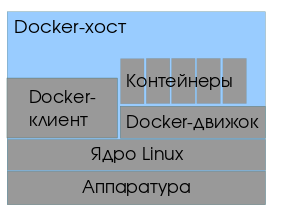
\includegraphics[width=0.8\textwidth]{images/docker.png}
  \caption{Docker на физическом Linux-сервере\label{docker}}
\end{figure}

Задумка контейнера – полная стандартизация. Контейнер соединяется с хостом
определенным интерфейсом, контейнеризорованное приложение не зависит от архитектуры
или ресурсов хоста. Для хоста же контейнер некий «черный ящик», не имеет значение что в нем.
На рисунке \ref{docker} приведена схема работы Docker на линуск сервере \cite{docker}.
Перечислим другие преимущества Docker:

\begin{itemize}[wide,topsep=0pt]
  \itemsep0em
  \item абстрагирование хост-системы от контейнеризованных приложений;
  \item простота масштабирования;
  \item простота управления зависимостями и версиями приложения;
  \item легкие, изолированные среды выполнения;
  \item совместно используемые слои;
  \item возможность компоновки и предсказуемость.
\end{itemize}

Таким образом, возможность быстрого развёртывания приложения на разных системах,
независимо от типа ОС, делает Docker крайне удобным инструментом для проектирования
нашего приложения.


\subsection{Python/Django}

При разработке программного обеспечения для серверной части был выбран
язык программирования Python совместно с Django.

Основные преимущества Python:
\begin{itemize}[wide,topsep=0pt]
  \itemsep0em
  \item Низкий порог вхождения: человеку, знакомому с программированием, достаточно получаса, чтобы начать писать на нем полезные для себя скрипты, а не знакомому – Python позволяет легко открыть для себя программирование и попробовать свои силы в нем.
  \item Хорошо спроектирован: Python вобрал в себя современные тенденции в программировании «с нуля». Кроме того, он динамично развивается: процесс включения новых конструкций в язык хорошо отлажен, и он продолжает впитывать в себя приемы функционального программирования, аспектно-ориентированного программирования и прочего, оставаясь при этом обратно-совместимым и внутренне непротиворечивым.
  \item Легко читаемый синтаксис (по сравнению с С++, Рerl, РНР): позволяет легко читать чужой код, разбираться в давно написанном собственном коде. В сочетании со сказанным выше это настраивает создателей библиотек на простоту и логичность интерфейсов.
  \item Огромное количество библиотек с кодом на любой случай жизни: будь то работа с таблицами Excel, изображениями или сетью Twitter.
  \item Переносимость: Python реализован под всеми распространенными операционными системами и на множестве архитектур – Windows, Linux, MacOS, даже на мини-компьютерах Arduino. Система зависимостей хорошо продумана, и разворачивание приложений на другой машине происходит легко и без сюрпризов.
\end{itemize}

Django - это свободный фреймворк для веб-приложений, использующий шаблон проектирования MVC.
Данный фреймворк является не только быстрым решением в веб разработке,
включающим все необходимое для качественного кода и прозрачного написания,
но также и отличной платформой для работы с клиентурой того или иного бизнеса,
а также разработчиков. С помощью Django можно гибко настроить панель управления контентом
(админку сайта) под любой конкретный проект - управление видеоматериалами,
комментариями и пользовательскими данными в данном случае.



\subsection{Очередь обработки видеофайлов}

Обработка видео является трудоемкой задачей, для которой требуется большое количество временных
и вычислительных ресурсов. Такого рода манипуляции не требуют участия конечного пользователя
вашего проекта, то есть их можно выполнять в фоновом режиме. При этом важно,
чтобы весь процесс оставался управляемым.

\begin{figure}
  \centering
  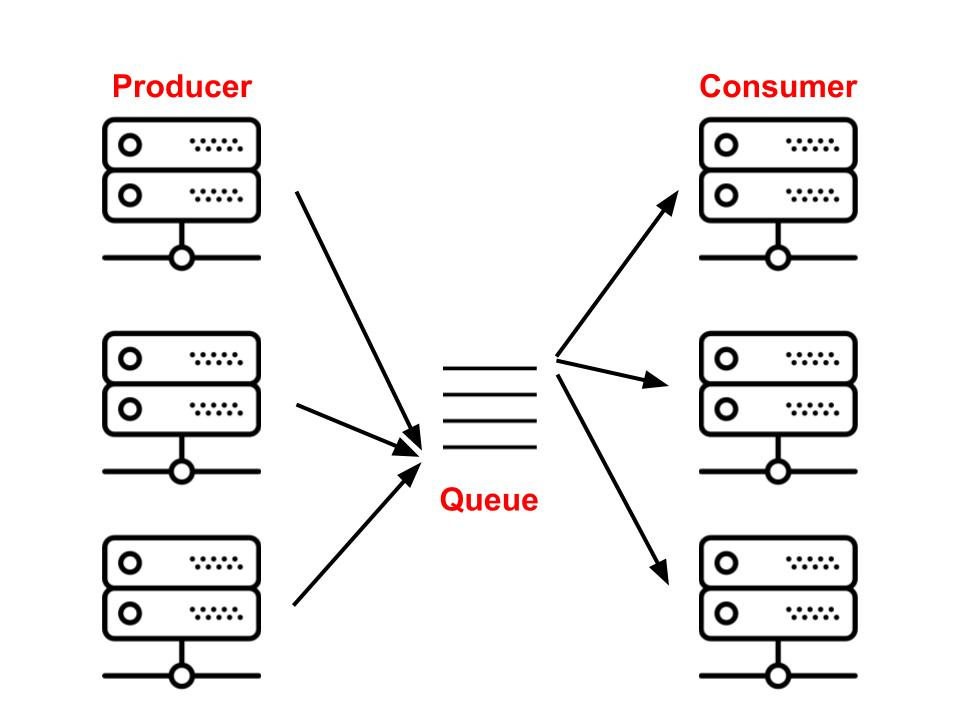
\includegraphics[width=0.8\textwidth]{images/producer-consumer.jpg}
  \caption{Очередь обработки видеофайлов\label{producer-consumer}}
\end{figure}

На рисунке \ref{producer-consumer} представлена общая схема очереди обработки видеофайлов.
Файлы, загруженные пользователями (“Producer” на схеме) из разных мест,
поступают в единую очередь “Queue”. Далее они обрабатываются обработчиками (“Сonsumer” на схеме)
в порядке поступления в очередь. Обработчик очереди может быть и один.
Для нашего приложения важно, чтобы очередь поддерживала следующий функционал:
\begin{itemize}[wide,topsep=0pt]
  \itemsep0em
  \item выполнение заданий асинхронно или синхронно;
  \item выполнение периодических заданий;
  \item выполнение задание повторно, если произошла ошибка;
  \item мониторинг выполнения заданий;
  \item проверка выполнения задания (уведомить пользователя о том, что видео прошло обработку).
\end{itemize}

В разработанном приложении было решено использовать распределенную очередь Celery,
которая является одним из самых популярных проектов для решения подобных задач в мире
python и Django. Это распределенная асинхронная очередь заданий, которая обладает
перечисленным выше функционалом, легко интегрируема и удобна в использовании.

\subsection{Content Delivery Network}

Скорость загрузки любого сайта достаточно важный и существенный параметр, который определяет
качество и надежность ресурса. Для образовательной платформы это вдвойне важно. При просмотре
видео не должны возникать существенные задержки в загрузке контента, иначе это негативно
скажется на общем впечатлении пользователей. Оптимизировать сайт можно многими способами,
и если каждый из них уже себя исчерпал, нужно подключать сторонние сервисы в помощь, например,
сервис CDN. Данная аббревиатура расшифровывается как Content Delivery Network – сеть доставки
контента. Чаще всего это множество серверов со специализированным ПО, которые ускоряют доставку
(“отдачу”) контента конечному пользователю. Сервера расположены по всему миру таким образом,
чтобы время ответа посетителям сайта было минимальным. Под “контентом” чаще всего
подразумевают видео и статические элементы веб-сайтов (не требующие выполнения кода на сервере
или запросов в базу данных, такие как css/js).

\begin{figure}
  \centering
  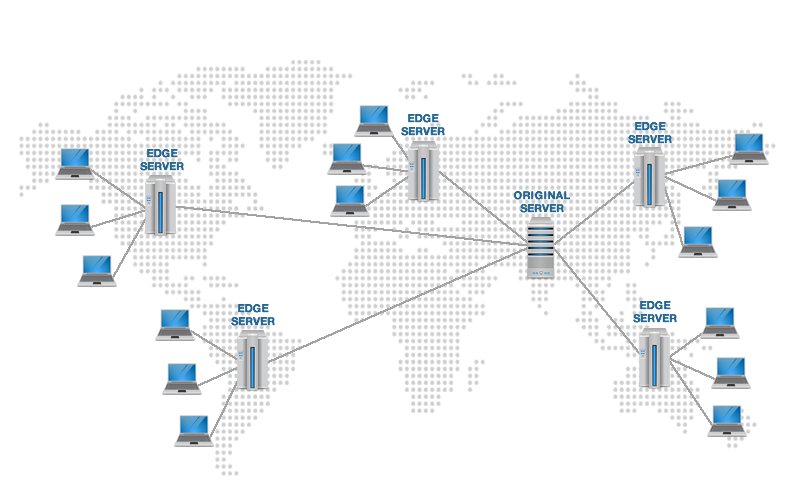
\includegraphics[width=0.9\textwidth]{images/how-cdn-works.png}
  \caption{Content Delivery Network\label{how-cdn-works}}
\end{figure}

На рисунке \ref{how-cdn-works} представлена одна из возможных схем распределения серверов CDN по миру.
Все современные CDN размещают копии контента на разных серверах по всему миру и направляют
клиента на ближайший (к клиенту) сервер. Результат — сокращение “latency”, то есть задержки
между запросом и ответом. Если на странице много изображений (пусть даже мелких картинок),
то чем быстрее они окажутся у клиента, тем быстрее клиент увидит страницу.

В разработанном приложении в качестве CDN было решено использовать Amazon CloudFront.
Это это удобный для разработчиков сервис глобальной сети доставки контента, обеспечивающий
быструю и безопасную передачу данных, видео, приложений и API клиентам по всему миру
с низкими задержками и высокой скоростью.

\subsection{JavaScript-фреймворк}

Выбор пал на AngularJS. AngularJS — JavaScript-фреймворк с открытым исходным кодом.
Предназначен для разработки одностраничных приложений. Его цель — расширение браузерных
приложений на основе MVC-шаблона, а также упрощение тестирования и разработки.
Фреймворк работает с HTML, содержащим дополнительные пользовательские атрибуты,
которые описываются директивами, и связывает ввод или вывод области страницы с моделью,
представляющей собой обычные переменные JavaScript. Значения этих переменных задаются
вручную или извлекаются из статических или динамических JSON-данных.

Ниже перечислим основные достоинства данного фреймворка, повлиявшие на выбор \cite{angular}.

\subsubsection*{Большое комьюнити}
В него входят как участники постоянной команды разработки,
так и просто те, кто хотят внести свою лепту в развитие фреймворка с открытым исходным
кодом. По Angular.JS проходит множество конференций, о нем говорят на хакатонах и спорят
в тематических ИТ-коммьюнити.
\subsubsection*{Декларативный стиль кода}
Это делает код более легковесным, облегчает его чтение и поддержку, так как
описывается необходимый конечный результат, а не все шаги по его достижению.
\subsubsection*{Использование директив}
В качестве языка шаблонов в Angular.JS используется HTML. Он расширяется с помощью директив,
которые добавляют в код сведения о требуемом поведении (например, о необходимости загрузить
определенный модуль сразу после загрузки страницы). Директивы позволяют вам сконцентрироваться
на проработке логики и работать более продуктивно. Их можно использовать повторно, что
также повышает читабельность кода.
\subsubsection*{MVC из коробки}
В AngularJS используется схема MVC, разделяющая логику, представление и данные приложения.
Cхема MVC показана на рисунке \ref{mvc}.
В Angular.JS имеется служба \$http, которая обеспечивает взаимодействие с удаленными
HTTP-серверами с помощью XMLHttpRequest или JSONP. При передаче объекта JavaScript
на сервер он будет автоматически преобразован в строку JSON. После получения ответа
служба также попытается преобразовать полученную строку JSON в JavaScript.
Используя службу \$http можно создать собственную службу с полным контролем над
обработкой URL и данных.

\begin{figure}
  \centering
  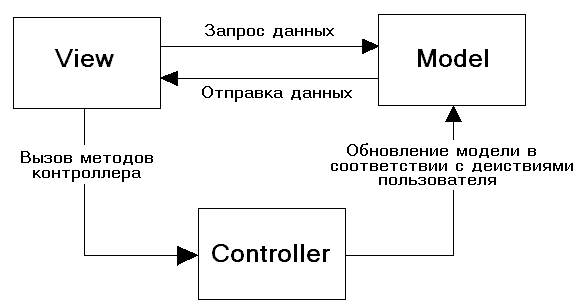
\includegraphics[width=0.9\textwidth]{images/mvc.png}
  \caption{Схема шаблона MVC\label{mvc}}
\end{figure}

\subsubsection*{Модульность}
В Angular.JS можно организовывать приложения из отдельных модулей. Такие модули
могут как зависеть друг от друга, так и быть автономными. Например, в последнем
случае модуль входа через Facebook можно использовать сразу в нескольких частях приложения,
скажем, на странице входа и на странице оформления заказа. А благодаря встроенному механизму
внедрения зависимостей Angular.JS сам распознает ситуацию, когда нужно предоставить
вспомогательные объекты, предоставляет их и связывает объекты между собой.
\subsubsection*{Наличие готовых решений}
Что важно, для Angular.JS существует огромное количество готовых решений, которые
позволяют решать довольно разнообразные задачи, используя уже готовые модули.
Например, существует несколько модулей для роутинга самый популярный из которых
ui-router, так же есть различные модули для работы с таблицами ui-grid, ng-table
и много других.
\subsubsection*{Простота тестирования}
Части приложения располагаются внутри модулей Angular.JS, которыми легко манипулировать.
Такая разбивка на модули позволяет загружать только нужные службы и эффективно выполнять
автоматическое тестирование. При этом если придерживаться принципа «один файл — один модуль»,
не будет возникать необходимости запоминать порядок загрузки модулей.
